\chapter{Metodologia}\label{cap:proposta}

Esta seção descreve a metodologia desenvolvida para comparar um conjunto de modelos de visão computacional, abrangendo tanto RNCs quanto ViTs, na tarefa de classificação da severidade da OA de joelho a partir de radiografias. A abordagem metodológica se baseia em quatro pilares principais: o uso de um conjunto de dados público, uma \textit{pipeline} de pré-processamento, a aplicação de \textit{transfer learning} para otimizar o treinamento dos modelos e uma avaliação robusta que abrange não apenas o desempenho preditivo, mas também a eficiência computacional, a quantificação de incerteza e a interpretabilidade dos modelos. Uma visão geral do processo é apresentada na \autoref{fig:metodologia}, que ilustra as etapas desde a coleta de dados até a avaliação final dos modelos.

\begin{figure}[ht]
    \centering
    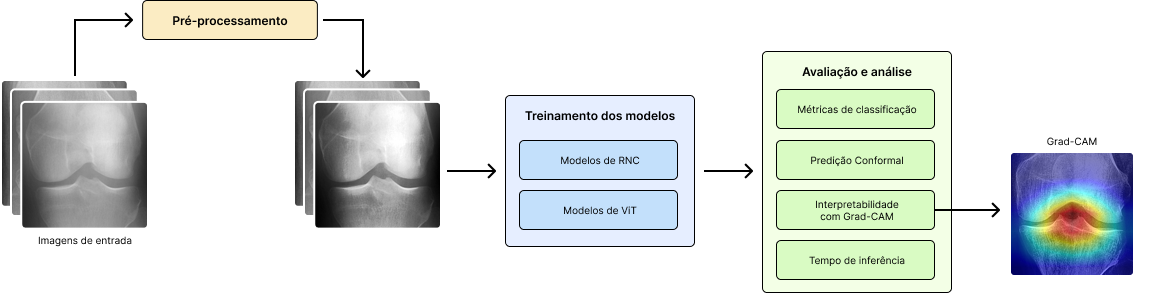
\includegraphics[width=\linewidth]{figs/metodologia-pgc.png}
    \caption{Visão geral da metodologia adotada neste estudo, desde a coleta de dados até a avaliação dos modelos.}
    \label{fig:metodologia}
\end{figure}

\section{Coleta de dados}

A base para qualquer modelo de aprendizado profundo é um conjunto de dados de alta qualidade. Para este estudo, foi utilizado o \textit{dataset} de radiografias de joelho da Osteoarthritis Initiative (OAI), obtido através da plataforma Kaggle \citep{dataset-kaggle}. Este conjunto de dados é amplamente utilizado na literatura científica \citep{Tariq2023, Mohammed2023} e consiste em 9.786 radiografias classificadas por especialistas segundo a escala de Kellgren-Lawrence (KL), cuja distribuição é detalhada na \autoref{dataset-summary}. A sua vasta dimensão e anotações confiáveis fornecem uma base sólida para o treinamento e a validação dos modelos.

\begin{table}[ht]
    \centering
    \begin{tabular}{|c|c|c|c|}
        \hline
        \textbf{Classe KL} & \textbf{Descrição} & \textbf{Total de imagens} & \textbf{\% do total} \\
        \hline
        0 & saudável & 3.857 & 40\% \\
        1 & duvidoso & 1.770 & 18\% \\
        2 & mínimo & 2.578 & 26\% \\
        3 & moderado & 1.286 & 13\% \\
        4 & severo & 295 & 3\% \\
        \hline
        \textbf{Total} & - & 9.786 & 100\% \\
        \hline
    \end{tabular}
    \caption{Número de radiografias por classe KL no conjunto de dados original.}
    \label{dataset-summary}
\end{table}

Todas as imagens possuem resolução de 224x224 pixels no formato PNG. Para garantir uma avaliação robusta, o conjunto de dados foi dividido em quatro subconjuntos distintos: treino (70\%), validação (10\%), teste (10\%) e calibração (10\%). Essa separação é uma prática recomendada que permite não apenas o treinamento (treino), o ajuste de hiperparâmetros (validação) e a avaliação final (teste) em dados não vistos, mas também a quantificação de incerteza (calibração), como detalhado na \autoref{sec:conformal-prediction}. A distribuição das classes em cada subconjunto é apresentada na \autoref{dataset-distribuition}.

\begin{figure}[ht]
    \centering
    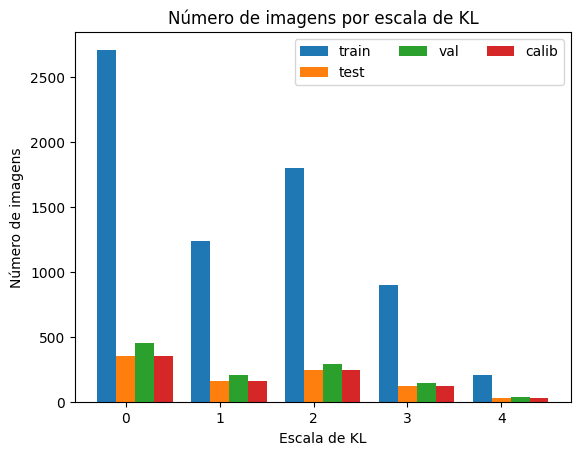
\includegraphics[width=0.7\linewidth]{figs/dataset-class-distribution.png}
    \caption{Distribuição das radiografias por classe KL nos subconjuntos de treino, teste, validação e calibração.}
    \label{dataset-distribuition}
\end{figure}

\section{Pré-processamento das imagens}

Uma \textit{pipeline} de pré-processamento foi aplicada para padronizar os dados e otimizar o aprendizado dos modelos. As técnicas foram aplicadas sequencialmente, visando aprimorar a qualidade da imagem e a robustez do treinamento.

Neste estudo, o pré-processamento das radiografias foi estruturado em duas etapas: uma etapa geral e outra específica para cada modelo. O pré-processamento geral, realizado antes do treinamento, envolveu técnicas simples como conversão para escala de cinza e equalização de histograma, com o objetivo de melhorar a qualidade das imagens. Por sua vez, o pré-processamento específico, executado durante o treinamento, consistiu na adaptação das imagens aos requisitos de entrada de cada modelo, incluindo operações como redimensionamento e normalização dos valores dos pixels. Adicionalmente, técnicas de aumento de dados foram empregadas para ampliar a variabilidade do conjunto de imagens e reduzir os efeitos do desbalanceamento entre as classes.

\subsection{Equalização de Histograma}

Para padronizar o contraste entre radiografias que podem ter sido obtidas com diferentes equipamentos e configurações, a equalização de histograma foi aplicada. Essa técnica redistribui a intensidade dos pixels, realçando detalhes sutis nas estruturas ósseas e no espaço articular, que são cruciais para a identificação de características da OA.

A implementação foi realizada com a biblioteca OpenCV \citep{opencv} do Python. A \autoref{fig:histogram-equalization}(a) ilustra uma radiografia original do joelho, enquanto a \autoref{fig:histogram-equalization}(b) mostra a mesma radiografia após a equalização de histograma. É possível observar que a equalização melhorou o contraste da imagem, tornando as estruturas ósseas mais visíveis. As respectivas distribuições de intensidade dos pixels antes e depois da equalização são apresentadas na \autoref{fig:histogram-equalization-histogram}.

\begin{figure}[ht]
    \centering
    \begin{tabular}{@{}c@{}}
        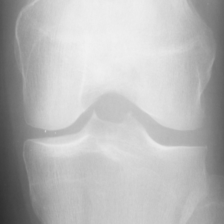
\includegraphics[width=0.35\textwidth]{figs/imagem-nao-equalizada.png} \\[\abovecaptionskip]
        \small (a) Radiografia original.
    \end{tabular}
    \hfill
    \begin{tabular}{@{}c@{}}
        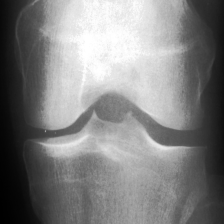
\includegraphics[width=0.35\textwidth]{figs/image-equalizada.png} \\[\abovecaptionskip]
        \small (b) Radiografia após equalização de histograma.
    \end{tabular}
    \caption{Exemplo de equalização de histograma aplicada a uma radiografia de joelho.}
    \label{fig:histogram-equalization}
\end{figure}

\begin{figure}[ht]
    \centering
    \begin{tabular}{@{}c@{}}
        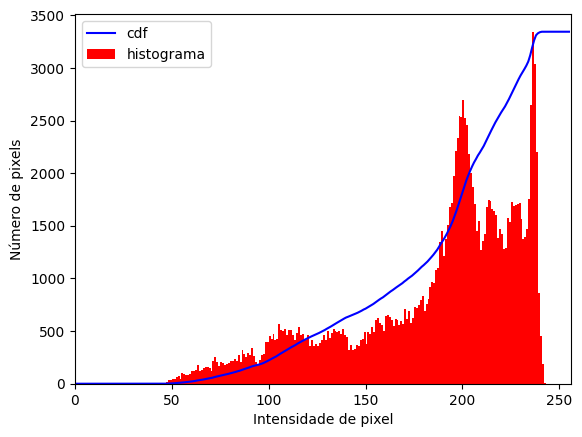
\includegraphics[width=0.45\textwidth]{figs/histograma-imagem-nao-equalizada.png} \\[\abovecaptionskip]
        \small (a) Histograma da radiografia original.
    \end{tabular}
    \hfill
    \begin{tabular}{@{}c@{}}
        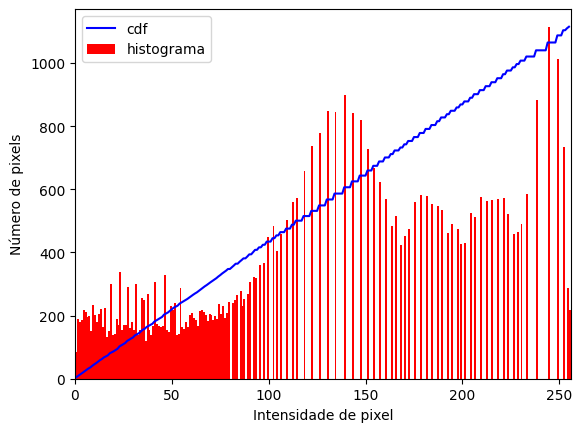
\includegraphics[width=0.45\textwidth]{figs/histograma-imagem-equalizada.png} \\[\abovecaptionskip]
        \small (b) Histograma da radiografia após equalização.
    \end{tabular}
    \caption{Distribuições de intensidade dos pixels antes e depois da equalização de histograma.}
    \label{fig:histogram-equalization-histogram}
\end{figure}

\subsection{Normalização}

A normalização dos valores dos pixels é um passo crítico para a eficácia do \textit{transfer learning}. Os valores de cada canal de cor foram padronizados para uma média de 0 e desvio padrão de 1.

Neste estudo, a normalização foi implementada em todos os subconjuntos de dados com a função \texttt{transforms.Normalize} da biblioteca PyTorch \citep{pytorch}, que aplica a normalização em cada canal (RGB), subtraindo a média e dividindo pelo desvio padrão. Para modelos RNC, como ResNet e VGG, utilizaram-se os valores convencionais para manter a compatibilidade com o pré-treinamento no ImageNet:

\begin{itemize}
    \item Média: 0.485, 0.456 e 0.406
    \item Desvio padrão: 0.229, 0.224 e 0.225
\end{itemize}

Para os ViTs, como o DeiT e o Swin Transformer, foram utilizados os valores específicos de normalização fornecidos por seus respectivos pacotes no Hugging Face.

\subsection{Aumento de dados}

Para aumentar a diversidade do conjunto de treinamento e mitigar o risco de \textit{overfitting}, foram aplicadas transformações geométricas aleatórias em tempo de execução. As técnicas incluíram a inversão horizontal (reflexão), com probabilidade de 50\%, e rotações leves limitadas a um intervalo de -10 a 10 graus. Essa estratégia expandiu artificialmente o \textit{dataset}, expondo o modelo a uma maior variedade de exemplos e melhorando sua capacidade de generalização, especialmente para as classes minoritárias.

Antes das transformações serem aplicadas, no entanto, as imagens foram redimensionadas para o tamanho esperado pelo respectivo modelo, definido como 224x224 pixels para todos os modelos, exceto para o modelo Inception-v3, que requer imagens de 299x299 pixels.

\subsection{Subamostragem}

O desbalanceamento de classes, evidente na \autoref{dataset-summary}, com a classe 0 (saudável) representando 40\% do total de imagens e a classe 4 (severo) apenas 3\%, pode enviesar o modelo em favor das classes majoritárias. Para combater isso, foi aplicada a técnica de subamostragem no conjunto de treino, limitando o número de amostras por classe a 1.700. Embora essa abordagem resulte na perda de alguns dados das classes majoritárias, ela foi escolhida por sua eficácia em forçar o modelo a dar igual importância a todas as classes, incluindo os estágios mais severos e menos frequentes da OA.

A técnica foi aplicada apenas no conjunto de treinamento, de modo a não comprometer a representatividade das distribuições nos conjuntos de validação, teste e calibração. Ela consistiu na seleção aleatória de um subconjunto das amostras das classes até um limite definido de 1.700 imagens por classe. Esse limite foi escolhido com base na classe 2 (mínima), que possui o maior número de imagens entre as classes com severidade, garantindo que todas as classes fossem representadas de forma equilibrada no conjunto de treinamento.

\section{Treinamento dos modelos}

A estratégia central de treinamento foi o uso de \textit{transfer learning} a partir de modelos pré-treinados no \textit{dataset} ImageNet-1K \citep{Russakovsky2015}. As arquiteturas, obtidas de repositórios como PyTorch e Hugging Face (\autoref{tab:model_list}), tiveram sua camada final de classificação substituída e adaptada ao número de classes esperado. A natureza do problema consiste em $K=5$ classes, correspondendo às categorias de severidade da OA de joelho, mas para a função de perda CORN o número de classes considerado foi $K-1$. Além disso, adotou-se a abordagem de ajuste fino (\textit{fine-tuning}), na qual todos os pesos da rede foram liberados para treinamento, permitindo que o modelo se adaptasse completamente às especificidades das imagens radiográficas.

\begin{table}[ht]
    \centering
    \begin{tabular}{|l|l|c|c|}
        \hline
        \textbf{Modelo} & \textbf{Fonte} & \textbf{Parâmetros (M)} & \textbf{FLOPs (GMac)} \\
        \hline
        ResNet-34 & PyTorch & 21,29 & 3,68 \\
        \hline
        ResNet-50 & PyTorch & 23,52 & 4,13 \\
        \hline
        ResNet-101 & PyTorch & 42,51 & 7,86 \\
        \hline
        VGG-16 & PyTorch & 138,36 & 19,63 \\
        \hline
        VGG-19 & PyTorch & 139,64 & 19,69 \\
        \hline
        DenseNet-121 & PyTorch & 6,96 & 2,9 \\
        \hline
        DenseNet-169 & PyTorch & 12,49 & 3,44 \\
        \hline
        Inception-v3 & PyTorch & 25,12 & 2,85 \\
        \hline
        DeiT-Distilled-Base & Hugging Face & 85,8 & 16,95 \\
        \hline
        DaViT-Base & PyTorch & 86,93 & 57,00 \\
        \hline
        MaxViT-Tiny & PyTorch & 30,41 & 5,48 \\
        \hline
        GCViT-Base & PyTorch & 89,30 & 13,89 \\
        \hline
        Swin-Base & PyTorch & 86,75 & 10,55 \\
        \hline
    \end{tabular}
    \caption{Lista dos modelos utilizados neste estudo, com a fonte, o número de parâmetros e FLOPs estimados.}
    \label{tab:model_list}
\end{table}

\subsection{Hiperparâmetros}

O treinamento foi realizado com os seguintes hiperparâmetros: otimizador Adam com taxa de aprendizado inicial de $1 \times 10^{-4}$, \textit{batch size} de 28 imagens, e um total de 60 épocas. Um agendador (\textit{scheduler}) reduziu a taxa de aprendizado por um fator de 10 a cada 5 épocas para refinar o ajuste dos pesos. Para evitar o \textit{overfitting}, foi implementado um mecanismo de parada antecipada (\textit{early stopping}) que monitorava a perda no conjunto de validação, com uma paciência de 5 épocas.

Reconhecendo a natureza inerentemente ordinal da escala KL, uma limitação frequentemente negligenciada em estudos de classificação, este trabalho adotou não apenas a função de perda \textit{cross-entropy} como linha de base, mas também a função CORN. Esta última reformula o problema de $K$ classes em $K-1$ tarefas de classificação binária (por exemplo, "a classe é maior do que 0?", "a classe é maior do que 1?", etc.), penalizando erros de forma proporcional à sua distância ordinal, o que é conceitualmente mais adequado para a classificação de severidade. Essa escolha metodológica permite uma avaliação mais justa e clinicamente relevante do erro do modelo.

O modelo com a melhor acurácia de validação foi salvo para a avaliação final. Por sua vez, ela foi conduzida no conjunto de teste, produzindo o relatório de métricas de classificação descrita na \autoref{sec:avaliacao-metricas}, além de gerar as matrizes de confusão e as curvas AUC-ROC para cada modelo. A complexidade computacional de cada arquitetura, em termos de FLOPs e quantidade de parâmetros, foi estimada com auxílio da bibliteca \textit{ptflops} \citep{ptflops}. Todos os resultados, incluindo métricas, tempos de execução e medidas de complexidade, foram armazenados em formato JSON para análise posterior.

\subsection{Ambiente de execução}

Todos os modelos foram executados na plataforma Google Colab, utilizando uma NVIDIA T4 GPU com 16 GB de memória, adequada para a tarefa de \textit{fine tunning} em modelos pequenos. A escolha dessa plataforma foi motivada pela sua acessibilidade e capacidade de fornecer recursos computacionais adequados a um custo reduzido.

\section{Avaliação e Análise Complementar}

Para ir além das métricas de desempenho tradicionais e abordar a necessidade crítica de confiança e transparência em sistemas de IA para medicina, a metodologia de avaliação foi enriquecida com três análises complementares: quantificação da incerteza das previsões, avaliação do tempo de inferência e interpretação das decisões dos modelos. Essas análises são fundamentais para entender não apenas o desempenho preditivo, mas também a aplicabilidade prática em cenários clínicos, diferenciando este estudo de outros trabalhos semelhantes.

\subsection{Predição Conformal}

Para quantificar a incerteza, foi aplicada a predição conformal. Em vez de uma única classe, essa técnica produz um conjunto de predição (por exemplo, \{1, 2\}) que é garantido conter a classe verdadeira com uma probabilidade especificada (neste caso, 95\%). Isso fornece uma medida de confiabilidade essencial para aplicações clínicas.

O conjunto de calibração foi usado para determinar os limiares de confiança para cada modelo. Para aqueles treinados com \textit{cross-entropy}, o limiar de confiança $\hat{q}$ foi calculado seguindo a abordagem descrita na \autoref{sec:conformal-prediction}, onde os \textit{scores} foram obtidos a partir das previsões do modelo. No entanto, para modelos treinados com o CORN foi adotada uma abordagem alternativa, tratando a saída da última camada como um conjunto de tarefas binárias ordenadas, que é exatamente como o CORN opera. Assim, para um problema com $K$ classes KL, a predição conformal sobre o CORN foi aplicada da seguinte forma:

\begin{itemize}
    \item Para cada exemplo do conjunto de calibração e cada $k \in \lbrace 0 \text{, } ... \text{, } K-2 \rbrace$ com probabilidade prevista $p_k$:
        \begin{itemize}
            \item Se $y_{\text{true}} > k$, $\text{score} = 1 - p_k$.
            \item Se $y_{\text{true}} \leq k$, $\text{score} = p_k$.
        \end{itemize}
    \item O limiar de confiança $\hat{q}_k$ foi calculado da mesma forma que na abordagem tradicional. Durante a inferência, para cada $k$, a classe $k+1$ foi adicionada ao intervalo de predição se $1 - p_k \leq \hat{q}_k$. Por exemplo, $\hat{y} \in [0,2]$ se apenas $k_0$ e $k_1$ estiverem acima do limiar de confiança.
\end{itemize}

\subsection{Análise do Tempo de Inferência}

A viabilidade de um modelo em um ambiente clínico depende não só da sua acurácia, mas também da sua velocidade. Para medir a eficiência prática, o tempo de inferência de cada modelo foi cronometrado. O processo foi repetido 50 vezes para cada arquitetura, e a média foi registrada, fornecendo uma métrica robusta para comparar a velocidade de predição em um cenário com hardware realista.

\subsection{Análise de Interpretabilidade com Grad-CAM}

Para promover a transparência e a confiança nos modelos, a técnica de visualização Grad-CAM foi utilizada. Ela gera mapas de calor que sobrepõem a radiografia, indicando quais regiões foram mais importantes para a decisão do modelo. Essas visualizações foram geradas para todos os modelos para permitir uma análise qualitativa, verificando se as arquiteturas estavam focando em áreas clinicamente relevantes (como o espaço articular) e comparando as diferenças entre os modelos RNC e ViT.

A implementação foi realizada com a biblioteca \textit{pytorch-grad-cam} \citep{jacobgilpytorchcam}, que facilita a aplicação do Grad-CAM em modelos treinados com PyTorch. As camadas escolhidas para a geração dos mapas de calor variou de acordo com a arquitetura do modelo, sendo as últimas camadas convolucionais para os RNCs e a última camada de atenção para os ViTs. A \autoref{tab:grad_cam_chosen_layers} resume as camadas selecionadas para cada arquitetura.

\begin{table}[ht]
    \centering
    \begin{tabular}{ll}
        \toprule
        \textbf{Arquitetura} & \textbf{Camada escolhida} \\
        \midrule
        ResNet & model.layer4[-1] \\
        VGG & model.features[-1] \\
        DenseNet & model.features[-1] \\
        Inception-v3 & model.Mixed\_7c \\
        DeiT-Distilled-Base & model.model.deit.encoder.layer[-1].layernorm\_before \\
        DaViT-Base & model.stages[3].blocks[0][1].norm1 \\
        MaxViT-Tiny & model.blocks[-1].layers[-1].layers[-1].attn\_layer[0] \\
        GCViT-Base & model.stages[-1].blocks[-1].norm2 \\
        Swin-Base & model.features[-1][-1].norm1 \\
        \bottomrule
    \end{tabular}
    \caption{Lista das camadas escolhidas para a geração dos mapas de calor Grad-CAM.}
    \label{tab:grad_cam_chosen_layers}
\end{table}

% \subsection{Otimização de Hiperparâmetros com Grid-Searching}

% Após uma rodada inicial de avaliação, os cinco modelos com melhor desempenho foram selecionados para uma fase de otimização de hiperparâmetros. Utilizando a biblioteca Optuna, um \textit{grid-search} foi executado para explorar sistematicamente diferentes combinações de taxa de aprendizado, \textit{batch size} e parâmetros do otimizador. O objetivo desta etapa foi refinar o treinamento dos modelos mais promissores para maximizar seu potencial preditivo.